\graphicspath{{./chapters/03/assets/}}

\chapter{Primo Progetto}
\label{cha:progetto1}
Il primo progetto sviluppato è stato scelto da parte del mio supervisore per permettermi di ambientarmi e apprendere i meccanismi generali di funzionamento delle tecnologie trattate nel Capitolo~\ref{cha:analisiTecnologie}, con particolare attenzione su AI Builder. 

Dietro a questa scelta si nasconde infatti una necessità da parte del team di sviluppo in quanto fino a quel momento non avevano mai avuto l'occasione per utilizzare AI Builder e quindi capirne potenzialità e limiti. In altre parole ho svolto il ruolo di ''cavia'' e al termire del progetto ho dovuto rendicontare riguardo alla mia esperienza in modo da decidere se AI Builder fosse uno strumento valido da utilizzare in progetti futuri. Il progetto da me svolto durante la prima fase dello stage infatti non era destinato al rilascio al cliente, anche se, nel caso in cui avesse avuto un riscontro positivo, avrebbe potuto essere proposto come estensione a ciò che l'azienda stava già sviluppando.

\section{Cliente e obiettivo}
Il cliente per cui è stato svolto il progetto è un'importante società di trasporti ferroviari inglese, il cui nome per questioni di riservatezza non è divulgabile. Questa società si occupa nello specifico della gestione e organizzazione degli interventi di controllo e manutenzione delle linee ferroviarie. Non si occupa tuttavia della realizzazione materiale degli interventi i quali vengono svolti da aziende partner.

Come si può facilmente ipotizzare la pianificazione di questi interventi è estremamente complessa, in quanto è necessario che diversi tasselli si incastrino: deviazione delle tratte ferroviarie, scelta dell'azienda che deve effettuare l'intervento, scelta di giornate e orari in cui effettuare i lavori, schieramento di mezzi e attrezzature, ecc...
Cluster Reply si è occupata quindi dello sviluppo di una soluzione software custom, basata su Microsoft Dynamics 365, che permettesse di semplificare e rendere più efficiente queste operazioni.

All'interno di questa soluzione, il mio ruolo è stato quello di automatizzare uno dei processi aziendali del cliente, senza però modificare le metodologie esistenti. 

\subsection{Processo Planning Request}
Dietro all'organizzazione di un intervento di controllo o manutenzione di trova configura un complesso ma ben delineato iter burocratico che fa pieno affidamento al CRM, dal momento in cui viene iniziato, fino alla sua conclusione positiva o negativa che sia.

Il processo è così composto:
\begin{enumerate}
  \item \textbf{Creazione della \textit{Planning Request}} - In seguito all'arrivo di un'email con uno specifico allegato, un addetto crea un record di tipo Planning Request mediante uno specifico form. E' anche possibile associare l'email ad una Planning Request esistente, ad un Contact o ad un Work Party. 
  \item \textbf{Approvazione della \textit{Planning Request}} - Composta da tre fasi:
  \begin{itemize} 
          \item Fase di pianificazione
          \item Fase di bozza
          \item Fase di pubblicazione
  \end{itemize}
\end{enumerate}

Una Planning Request è l'entità su cui questo processo è costruito. Essa è basata sull'entità standard Incident del CRM, su cui sono state effettuate diverse modifiche in modo da adattarla alle necessità del caso. In sostanza, sono stati aggiunti diversi campi e associazioni con altre entità come, ad esempio, l'entità Job, la quale invece modella una attività che deve essere eseguita da un Work Party, entità che rappresenta un'azienda partner.
La customizzazione del CRM per questo cliente comprende inoltre altre funzionalità di importanza marginale per questa trattazione.

L'obiettivo del progetto che mi è stato assegnato è quello di automatizzare la prima fase e parte della seconda, ovvero la creazione della Planning Request e la sua pianificazione. Essendo infatti una semplice operazione di trascrizione del contenuto dell'allegato nel sistema, la sua automatizzazione permetterebbe il risparmio di molto tempo per i dipendenti del cliente.

Per la realizzazione del progetto quindi è stato scelto di creare un flusso cloud Power Automate per la creazione e la pianificazione della Planning Request a partire dai dati estratti dall'allegato mediante un modello di elaborazione di moduli di AI Builder opportunamente creato e allenato.

\subsection{Creazione Planning Request in dettaglio}
La processo di creazione di una Planning Request inizia in seguito all'arrivo di una email indirizzata ad un apposita casella di posta. Le email inviate a questo indirizzo vengono automaticamente assegnate a una Coda (\textit{Queue}) del CRM, chiamata Power Planning Queue. Le email iniviate a questo indirizzo devono avere in allegato un documento appositamente compilato, in Figura~\ref{fig:planningRequestDocument} un esempio.
\begin{wrapfloat}{figure}{I}{0pt}
  \centering
  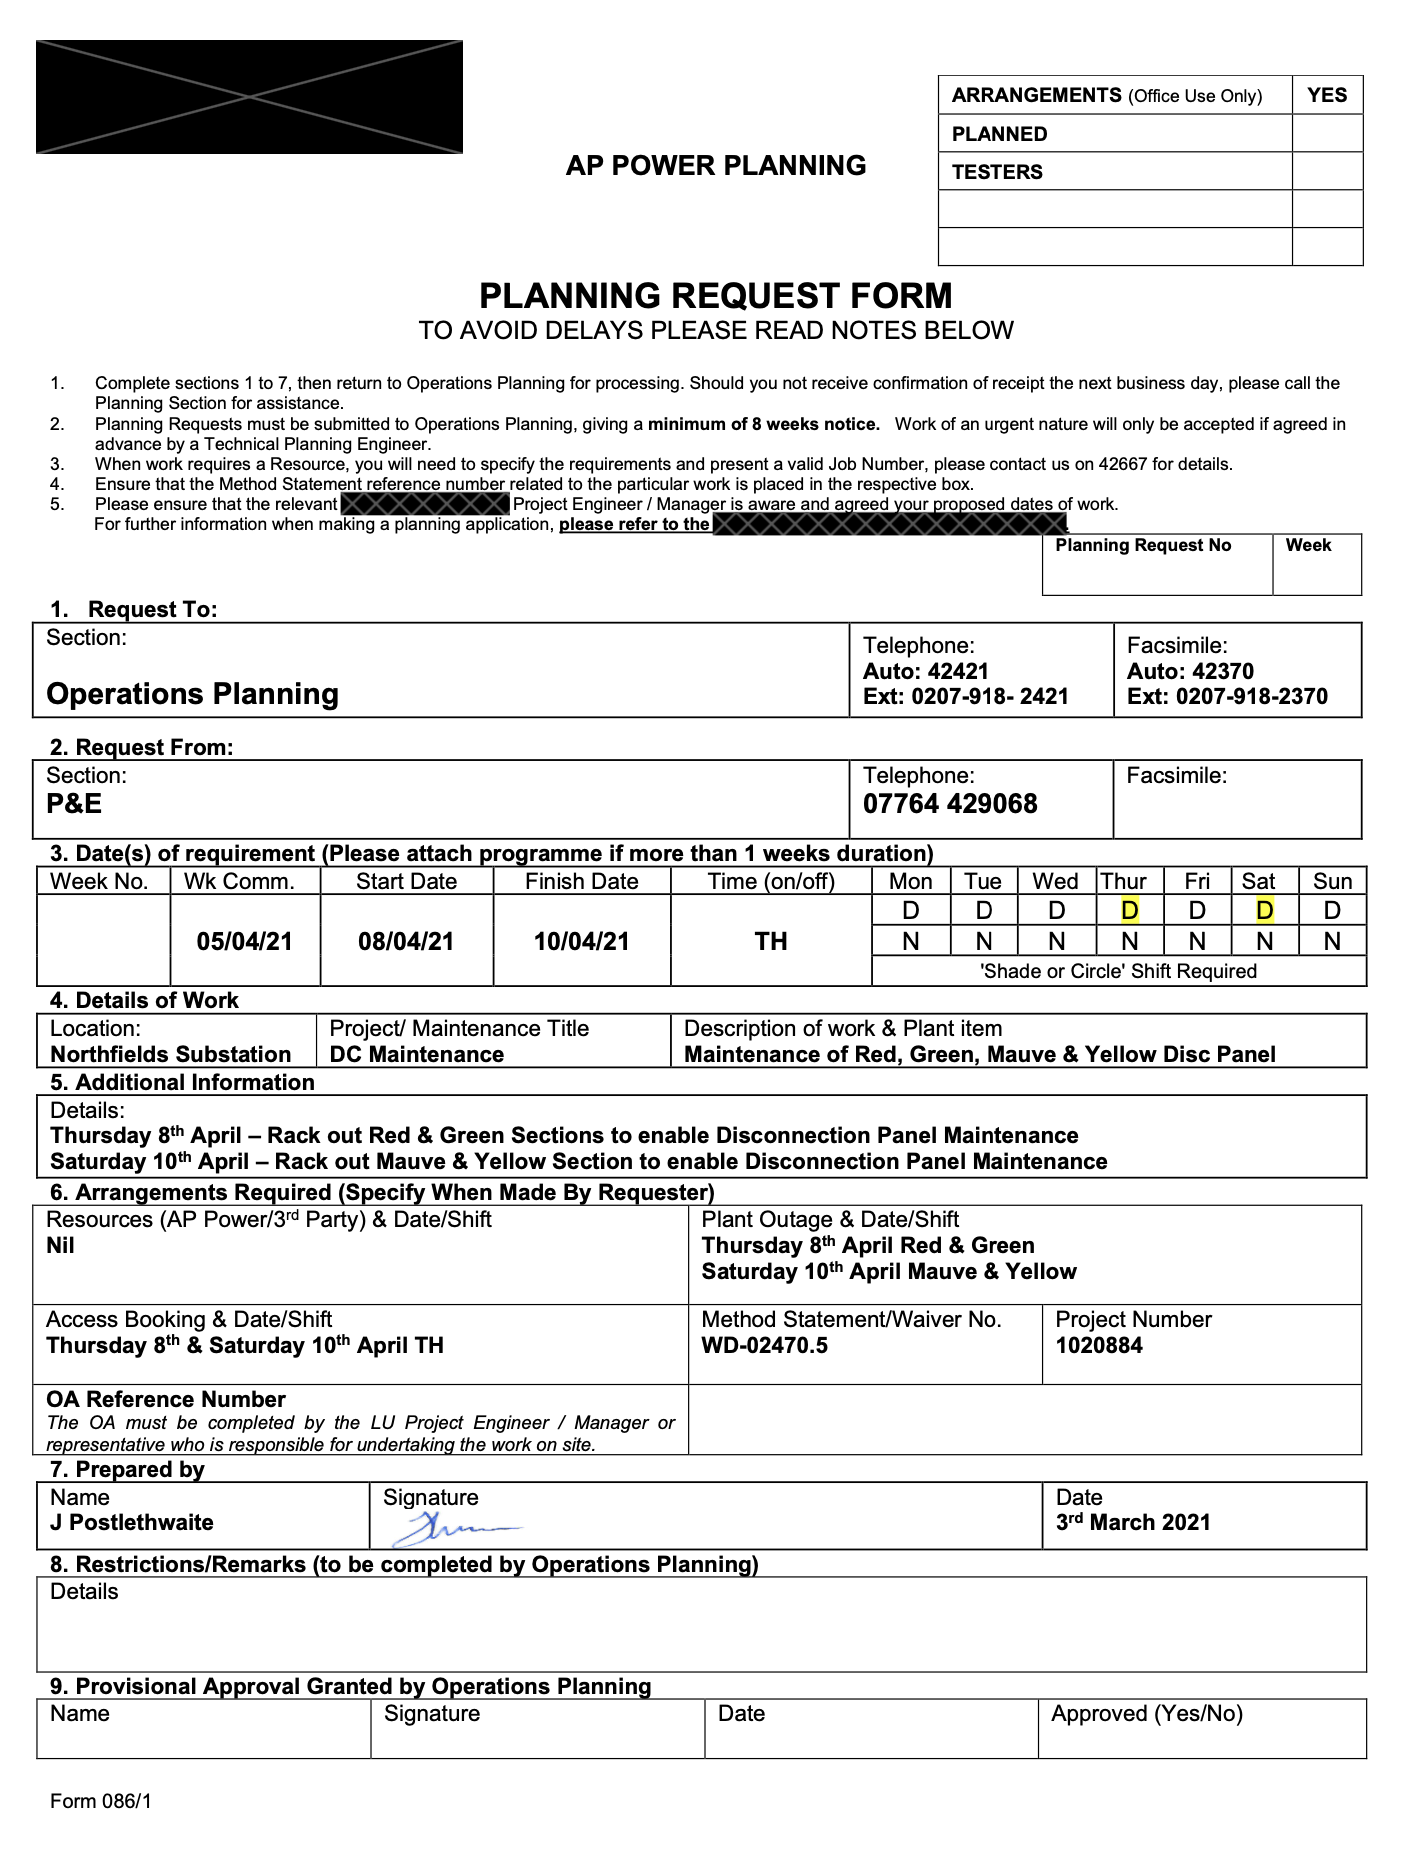
\includegraphics[width=0.5\textwidth]{planning-request-document.png}
  \caption{Esempio di documento Planning Request}
  \label{fig:planningRequestDocument}
\end{wrapfloat}

Se per qualche motivo il documento viene inviato in maniera fisica (ad esempio mediante fax o posta), l'addetto si dovrà occupare di scannerizzarlo e inviarlo alla Power Planning Queue.


Per la creazione di una Planning Request viene sfruttata la funzionalità standard di promozione di un elemento di una Queue in un altro record (come ad esempio un Lead). In questo modo la Planning Request creata erediterà le informazioni, ad esempio il contatto, dall'email e avrà l'email in questione come Activity associata. 
Il sistema inoltre consente di creare una Planning Request anche senza partire da un elemento di una coda. In questo caso sarà l'addetto a dover inserire manualmente le informazioni richieste. 

Una Planning Request appena creata entra in fase di approvazione. Le entità del CRM con cui si ha a che fare durante questa fase del processo sono: 
\begin{itemize}
  \item Planning Requests
  \item Jobs \begin{itemize}
    \item Job Schedules 
    \item Job Resources
    \item Work Documents
    \item Job Arrangements
    \item Job Outages
  \end{itemize}
\end{itemize}

Senza entrare nel dettaglio di come sono costituite queste entità è importante sapere le relazioni esistenti tra esse: Jobs è in relazione con Planing Request mentre Job Schedules, Job Resources, Work Documents, Job Arrangements e Job Outages sono in relazione con Jobs. 

L'addetto ha il compito di compilare manualmente i campi di queste entità sulla base del contenuto del documento allegato all'email che inizia il processo di creazione di una Planning Request. 
Ciò che mi è stato chiesto di fare è di automatizzare quanto più possibile del processo appena visto in modo da ridurre al minimo l'intervento umano.

\section{Sviluppo del progetto}
Lo sviluppo è stato diviso in due fasi: 
\begin{itemize}
  \item Creazione e training del modello AI Builder per la raccolta automatica dei dati dal documento.
  \item Sviluppo del flusso cloud Power Automate.
\end{itemize}
  
\subsection{Modello AI Builder}
Per l'estrazione automatica dei dati dal documento è stato scelto di utilizzare il modello personalizzato di elaborazione di moduli di AI Builder. 

Per prima cosa è stato necessario definire quali dati raccogliere. Il mio supervisore ha specificato che era sufficiente raccogliere i seguenti:
\begin{itemize}
  \item Work Type
  \item Work Party
  \item Resources
  \item Location
  \item Originator Reference
  \item Description
  \item Comment
  \item Schedule (tabella che specifica giorni e fasce orarie di lavoro)
\end{itemize}
Dopo aver scaricato dal database del CRM un dataset di \num{500} documenti compilati appartenti a Planning Request già esistenti, ho effettuato un'estrazione casuale di \num{20} documenti mediante un semplice script python e li ho utilizzati come training set per il modello AI Builder, completando la fase di etichettatura manuale descritta in Sezione~\ref{ssec:creazioneModello}. Il numero di documenti scelto per il training è stato di \num{20} documenti per trovare un compromesso tra il tempo necessario all'etichettatura e il rischio di \textit{overfitting}. 

\subsubsection{Problematiche incontrate}
Sono state rilevate diverse problematiche nell'utilizzo del modello.
Sebbene il training fosse stato effettuato su un campione di documenti eterogeneo nei contenuti ma con la stessa struttura, il modello ha manifestato cattiva performance in caso di documenti con campi dimensionati o posizionati diversamente, anche se in maniera lieve, rispetto ai documenti utilizzati per il training.

Particolare attenzione è stata dedicata, inoltre, alla tabella \textit{Schedule}, che è risultata difficile da trattare a causa delle limitazioni di AI Builder. Come spiegato in Sezione~\ref{sssec:esempioModello}, non è supportato il riconoscimento di caselle di controllo, funzionalità che sarebbe stata proprio quanto necessario per la corretta estrazione dei dati dalla tabella. Essa infatti viene compilata evidenziando, cerchiando o annerendo la cella desiderata. Estrarre dalla tabella giorni e fasce orarie desiderate è risultato pertanto impossibile.

Non potendo intervenire su AI Builder, ho tentato strade alternative apportando modifiche ai documenti stessi e creando nuovi modelli allenati su dataset appositamente preparati. In Figura~\ref{fig:tabelleConSenzaMod} alcuni esempi.

Nonostante questi tentativi nei documenti forniti per il testing la tabella \textit{Schedule} non veniva mai correttamente rilevata. Nel caso del tentativo basato sull'annerimento totale della cella desiderata, essendo il riconoscimento di caselle di controllo non supportato, era facilmente prevedibile che ciò non avvenisse.
Il tentativo con i caratteri 'X' invece si basava sull'assunto che il modello è pensato per il riconoscimento di campi testuali e quindi avrebbe potuto avere successo nel rilevare i caratteri 'X' nelle celle corrispondenti. Anche questo tentativo non ha avuto successo in quanto le tabelle non venivano rilevate affatto (oggetto JSON di output vuoto).

\begin{figure}
  \centering
  \subfloat[][\emph{Tabella senza modifiche.}]
     {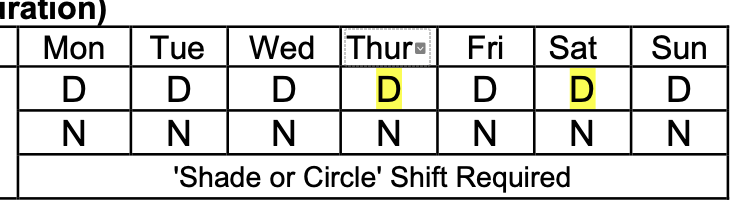
\includegraphics[width=.45\textwidth]{schedule-nomods1.png}} \quad
  \subfloat[][\emph{Altra tabella senza modifiche.}]
     {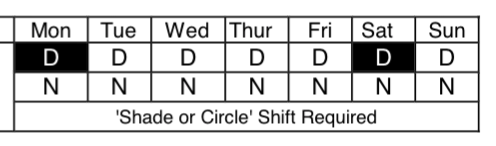
\includegraphics[width=.45\textwidth]{schedule-nomods2.png}} \\
  \subfloat[][\emph{Tabella modificata con annerimento totale.}]
     {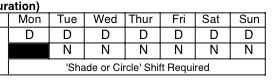
\includegraphics[width=.45\textwidth]{schedule-black.png}} 
     \quad
  \subfloat[][\emph{Tabella modificata con carattere 'X'.}]
     {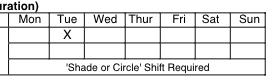
\includegraphics[width=.45\textwidth]{schedule-cross.png}} 
  \caption{Esempi di tabelle con e senza modifiche.}
  \label{fig:tabelleConSenzaMod}
\end{figure}

È stato deciso dunque di ignorare la tabella \textit{Schedule} e quindi evitare poi di compilare i campi dell'entità Job Schedule ad essa corrispondente. La parte di processo che ho dovuto automatizzare si ferma dunque alla creazione del Job.

\subsection{Flusso Power Automate}
Lo sviluppo del flusso cloud su Power Automate è stato abbastanza semplice e diretto e non ho riscontrato grosse difficoltà. In Figura~\ref{fig:flussoTfl} è presente il flusso completo mentre in Figura~\ref{fig:bloccoPlanningRequest} è presente il blocco di creazione del record Planning Request.

\begin{figure}[ht]
  \centering
  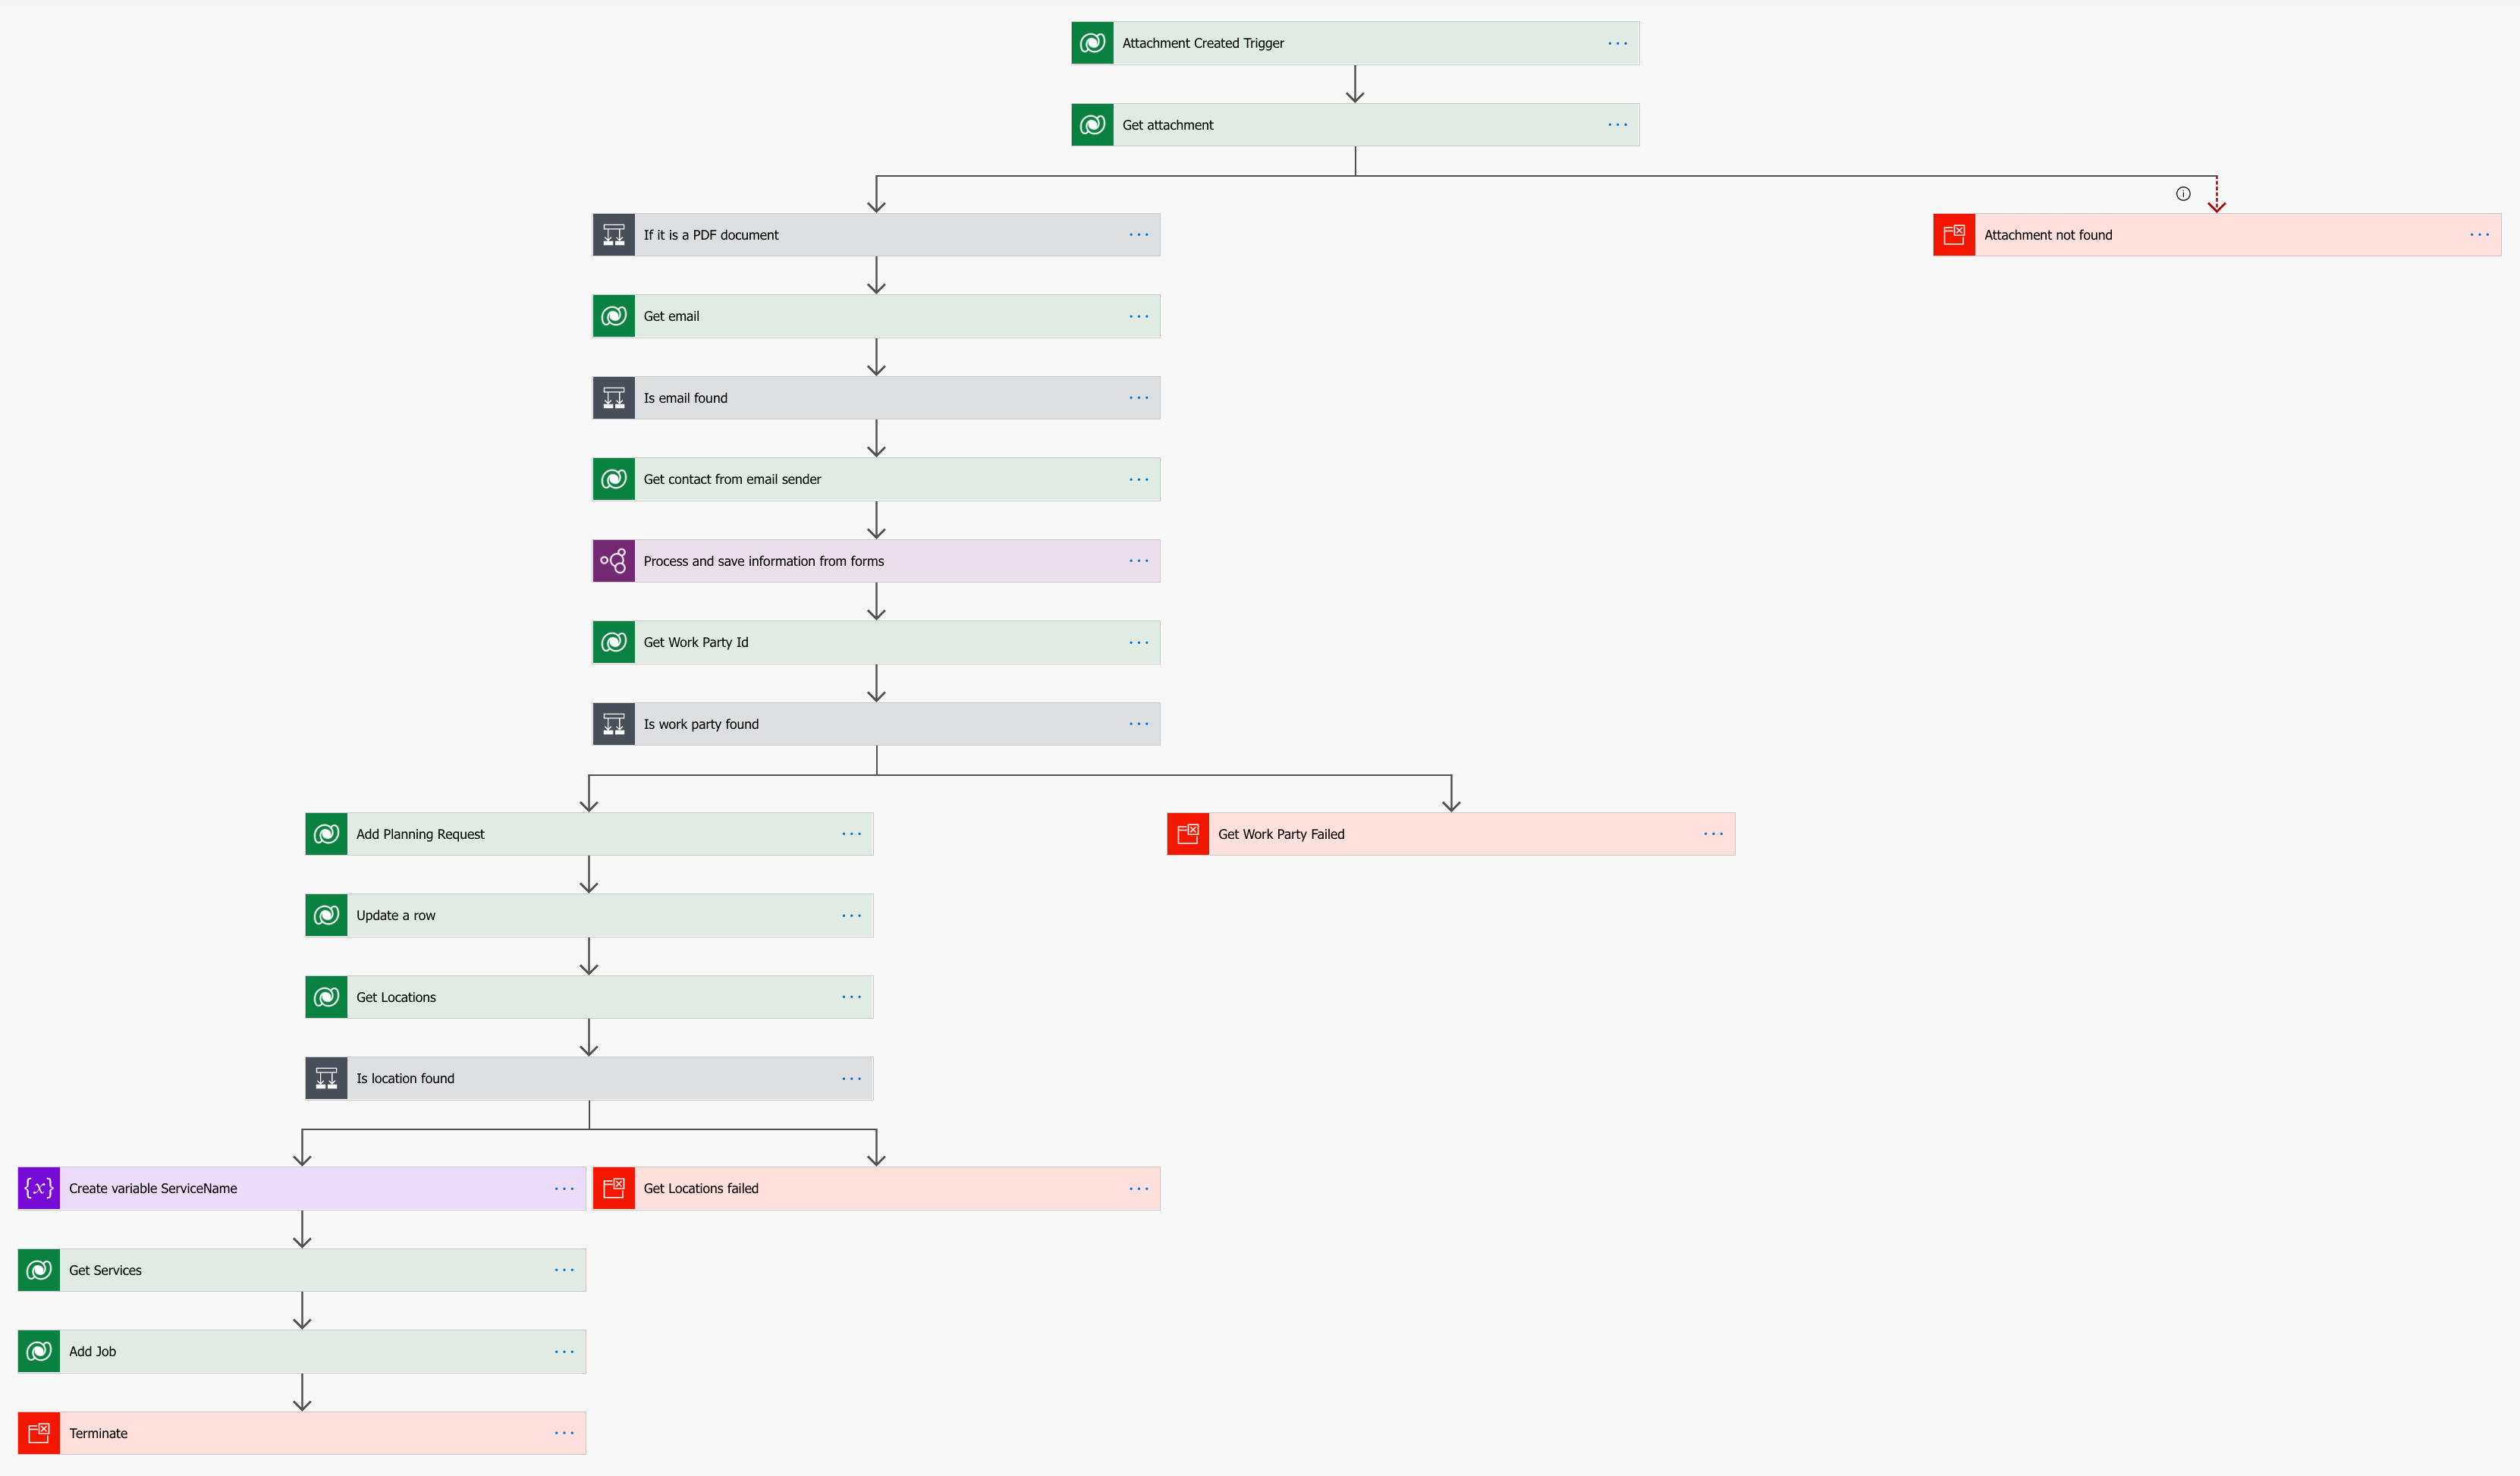
\includegraphics[width=\textwidth]{flusso-cloud-tfl.png}
  \caption{Flusso cloud Power Automate per l'automatizzazione della creazione di Planning Request.}
  \label{fig:flussoTfl}
\end{figure}

\begin{figure}[ht]
  \centering
  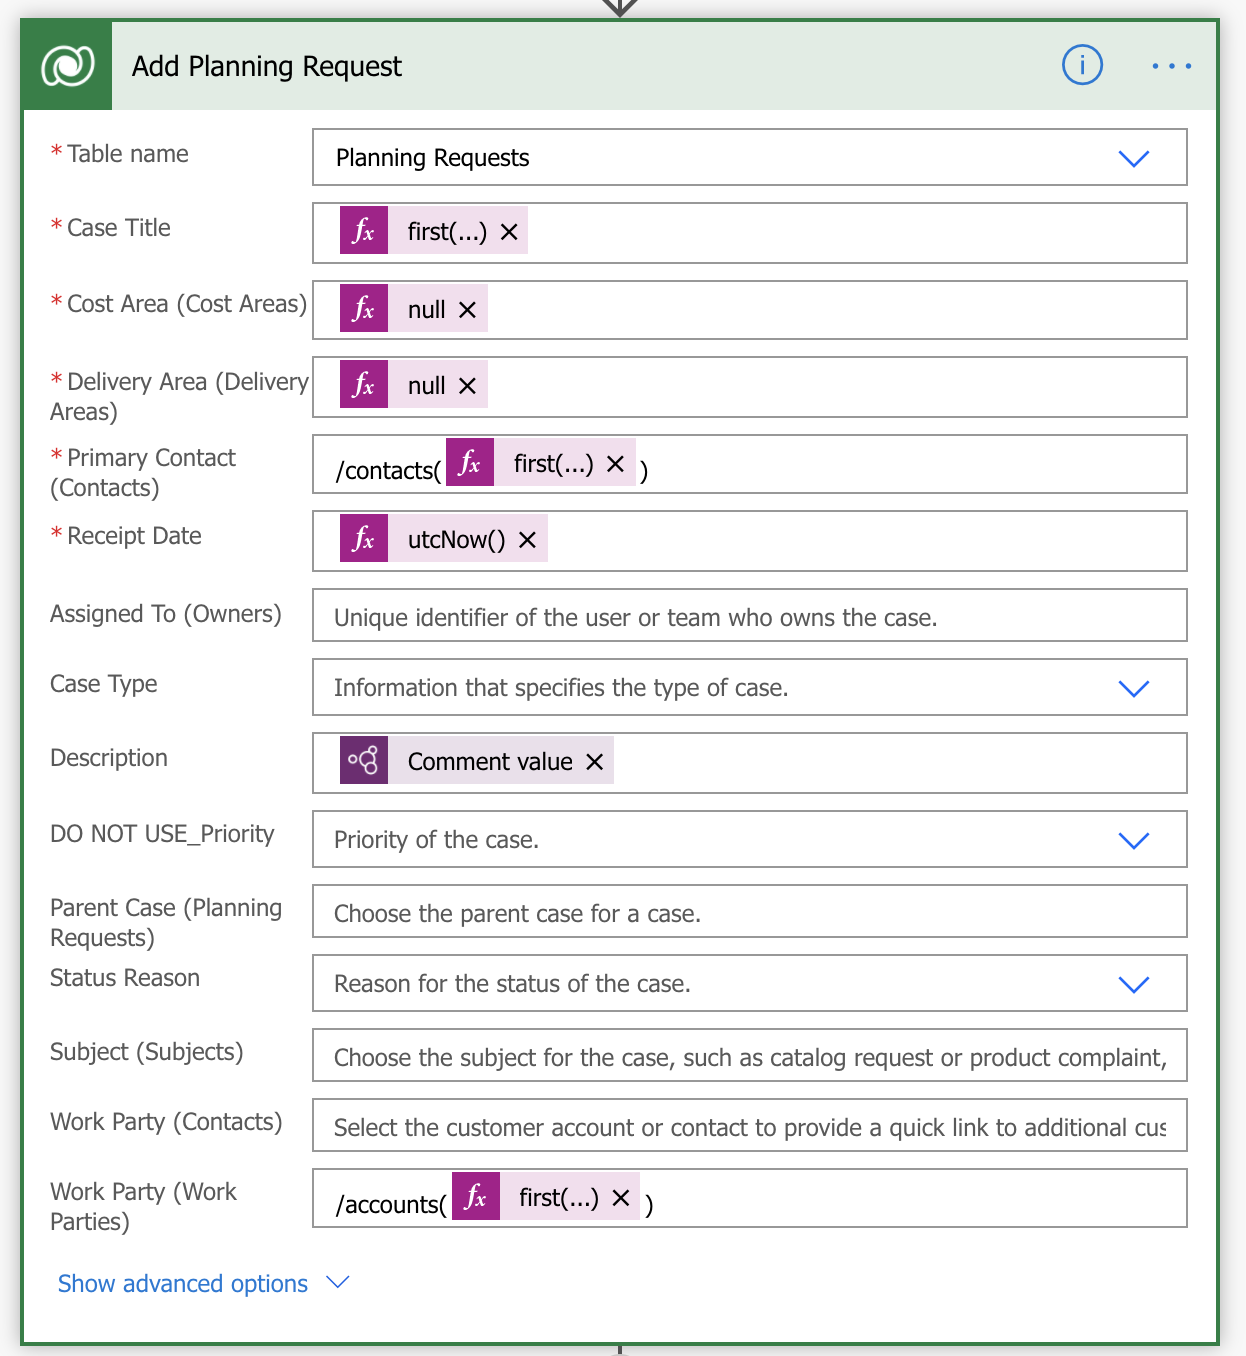
\includegraphics[width=0.6\textwidth]{planning-request-block.png}
  \caption{Blocco di creazione di una Planning Request.}
  \label{fig:bloccoPlanningRequest}
\end{figure}
Il flusso si compone di diverse fasi:
\begin{enumerate}
  \item Trigger sulla creazione di un record Attachment nel CRM, controllo che l'allegato che ha attivato il trigger sia di tipo PDF e controllo che l'allegato in questione sia in relazione con un record Email.
  \item Elaborazione del documento mediante AI Builder
  \item Ottenimento dell'ID univoco del Work Party da associare alla Planning Request, a partire dal valore estratto dal documento.
  \item Creazione di un record Planning Request e aggiornamento del campo Regarding della email per cui il flusso è in esecuzione, in modo da associare l'email alla Planning Request.
  \item Ottenimento dell'ID univoco della Location da associare al Job relativo alla Planning Request, a partire dal valore estratto dal documento.
  \item Ottenimento dell'ID univoco del Service da associare Job relativo alla Planning Request, a partire dal valore estratto dal documento.
  \item Creazione del Job, utilizzando i dati ottenuti in precedenza e quelli estratti dal documento.
\end{enumerate}


